\documentclass[a4paper,12pt]{article}
\author{}
\date{}
\usepackage[papersize={216mm,330mm},tmargin=20mm,bmargin=20mm,lmargin=20mm,rmargin=20mm]{geometry}
\usepackage[utf8]{inputenc}
\usepackage{amsmath,amssymb,mathabx}%\for eqref
\usepackage{lscape}
\usepackage{graphicx}
\usepackage[colorinlistoftodos]{todonotes}
\usepackage{fancyhdr}
\usepackage{subcaption}
\usepackage{comment}

\graphicspath{{./imagenes/}}
 
\pagestyle{fancy}
\fancyhf{}
\lhead{Universidad de Monterrey}
\chead{\thepage}
\rhead{Facultad de Ciencias Fisico Matemáticas}
\lfoot{Mediciones y Metrología}
\cfoot{Actividad 4 - Calorimetría}
\rfoot{Rolando Rivas Dávalos}

\title{\Large \textbf{Universidad de Monterrey}\\ Facultad de Ciencias Fisico Matemáticas \\ Mediciones y Metrología \\ 
\includegraphics{imagenes/UdemLogo.png} \\ \vspace{5mm} \LARGE \textbf{Actividad 4 - Calorimetría} \\ \vspace{1cm} \normalsize por \\ \vspace{1cm} \Large \textit{Rolando Rivas 594276}}

\begin{document}
\maketitle
\section*{Introducción}
A lo largo de toda la historia de ciencia se han usado conceptos abstractos para estudiar el mundo físico y sus fenómenos como la \textbf{energía} ($J$). Esta surge de la observación directa de los fenómenos físicos y su posterior abstracción en formas cuantificables. Una de las notables propiedades que posee la energía es su conservación; no se crea ni se destruye, solo se transforma a sus diferentes formas. Varias de estas formas incluyen la Energia mecánica, nuclear, termica, electromagnética, etc.

La energia térmica se define como la cantidad de energia en forma de calor en un sistema cerrado. El calor a nivel atómico realmente es la velocidad a la que las particulas vibran, por lo tanto es un tipo de energía cinética. Sin embargo por obvias razones es casi imposible medir cada particula individual por lo que se recurre a medir el conjunto de las vibraciones, la \textbf{temperatura}.

La temperatura es una escala medida en grados y no en Joules ($J$) ya que tiene sus bases en fenomenos fisicos (El grado 0 en Celcius es la temperatura de congelación del agua). Si se quiere modelar el cambio de temperatura ($\Delta T$) en terminos de Joules se necesitará una unidad que relacione estas dos. El \textbf{calor específico} ($c$) es la unidad que equivale a Julios por Kilogramo ($m$) por Kelvin. 

Ejemplos de materiales y su calor especifico:
\begin{itemize}
    \item Latón: $350 \frac{J}{kgK}$
    \item Aluminio: $900 \frac{J}{kgK}$
    \item Cobre: $390 \frac{J}{kgK}$
    \item Agua: $4,186 \frac{J}{kgK}$
\end{itemize}

El calor especifico representa cuantos Joules de energía se necesitan para calentar cierta cantidad de un material 1 grado. Esto da a lugar una ecuación que predice cuanto calor ($Q$) entró o salió ($\Delta T$) de un cierto material ($c$) con una cantidad especifica de masa ($m$). Esto da a lugar la ecuación
\[Q = mc\Delta T\]
\\
donde $Q$ es la energía entrante (si es positiva) o saliente (si es negativa). La razón por la que se dice que la energía "entra" o "sale" es debido a la segunda ley de la termodinámica. Esta postula que la energía siempre se conserva transformandose de un tipo a otro.
\\
\subsection*{Objetivo}
El proposito de esta actividad es la de familiarizarse con los conceptos de calor específico y conservación de energía. Se medirá en un experimento el cambio de temperatura del agua al ser sometido a un solido caliente y se derivarán los valores de capacidad calorifica de los metales para su análisis.
\\
\section*{Materiales y Métodos}
Los materiales usado para hacer el experimento son:
\begin{itemize}
    \item Termómetro
    \item Agua en un contenedor
    \item Cobre, Aluminio y Latón 
    \item Báscula
    \item Temporizador
\end{itemize}
Se iniciará manteniendo las variables de las masas (del metal y del agua) constantes, dado un valor inicial. Tambien se le dará valor inicial a las temperaturas de los antes mencionados, las cuales cambiarán una vez entren en contacto. Se inserta entonces el metal caliente dentro del agua y se medirá su cambio de temperatura. Se registrarán los resultados.

\section*{Resultados}
A continuación se muestran las gráficas Temperatura vs Tiempo de los tres metales.

\begin{figure}[h]

\centering
  \subcaptionbox{Cobre \label{fig:grafica1}}
  {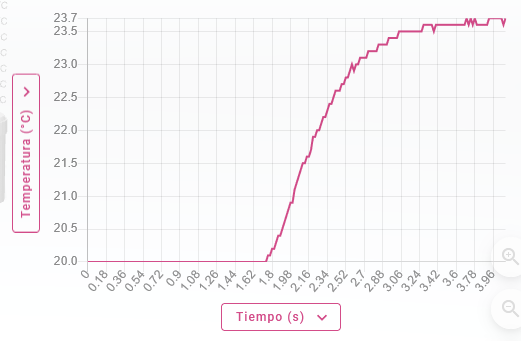
\includegraphics[width=0.3\textwidth]{imagenes/cobre.png}}
  \hfill
  \subcaptionbox{Latón \label{fig:grafica2}}
  {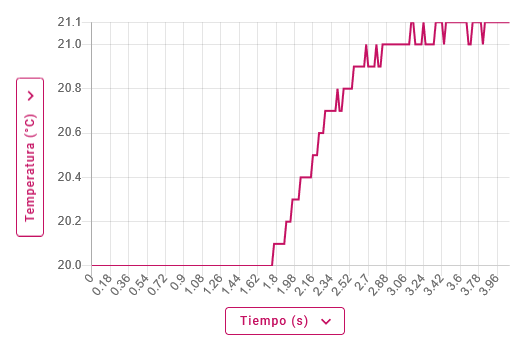
\includegraphics[width=0.3\textwidth]{imagenes/laton.png}}
  \hfill
  \subcaptionbox{Aluminio \label{fig:grafica3}}
  {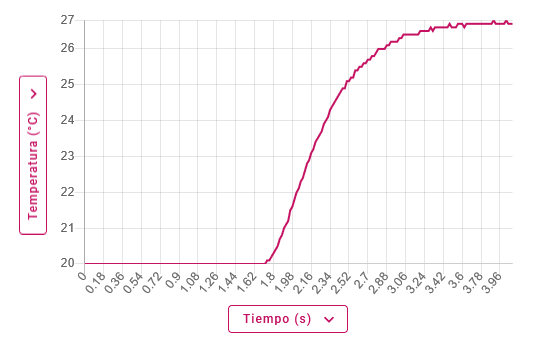
\includegraphics[width=0.3\textwidth]{imagenes/aluminio.png}}
  \caption{Observando las gráficas las tres muestran un rápido crecimiento de la temperatura en el segundo 1.78 que resulta del primer contacto del agua con el metal. Se puede apreciar que tasa de cambio de la temperatura va disminuyendo con el tiempo y se equilibra en un valor.}
\end{figure}


Durante el experimento se mantivieron constantes las variables de la masa y temperaturas iniciales del agua ($m_{a}$ y $T_{ia}$ respectivamente) y de los metales ($m_{m}$ y $T_{im}$). Tambien se midió el cambio de temperatura del agua y los metales ($\Delta T_{a}$ y $\Delta T_{m}$). Tomando como referencia la capacidad calorífica del agua ($c_{a}$) se calculará la capacidad calorífica de los metales ($c_{m}$) con ayuda de las variables antes mencionadas. Finalemente $c_{m}$ será comparada con su valor teórico real. 



\begin{table}[h!]
\centering
 \begin{tabular}{||c c c c c c c c c c c c||} 
 \hline
 $c_{a}$ & $m_{a}$ & $T_{ia}$ & $\Delta T_{a}$ & $m_{m}$ & $T_{im}$ & $\Delta T_{m}$ & $T$ & $c_{m}$ (exp) & $c_{m}$ (teo) & error & Metal \\ [0.5ex] 
 \hline\hline
 4186 & 0.15 & 20 & 1.1 & 0.0668 & 50 & 28.6 & 21.1 & 361.53 & 350 & 3.2857 & Latón \\
 4186 & 0.10 & 20 & 3.7 & 0.0701 & 80 & 56.3 & 23.7 & 392.44 & 390 & 0.6256 & Cobre \\ 
 4186 & 0.05 & 20 & 6.7 & 0.0212 & 100 & 73.3 & 26.7 & 902.41 & 900 & 0.2678 & Aluminio \\[1ex] 
 \hline
 \end{tabular}
 \caption{Datos de la temperatura, masa y calor especifico de los metales medidos. }
\end{table}

%\section*{Discusiones}

\section*{Conclusiones}
Los errores obtenidos al comparar calor especifico teórico y experimental de los metales son relativamente bajos y precisos. Cada material tiene su propio calor específico teniendo los metales una capacidad mayor de transferencia de calor comparado con otros metales.

\section*{Referencias}
Fisica Universitaria (12th ed., Vol. 1). (2009). [Pdf]. PEARSON EDUCACIÓN.

\textit{Doy mi palabra que he realizado esta actividad con integridad académica}

\end{document}